
\par
W tej sekcji wyjaśniona jest ogólna struktura programu, z pominięciem dokładnych opisów poszczególnych elementów.
Ich szczegółowy opis znajduje się w następnych sekcjach.
\par
Obiekt okna, klasy \sokarclass{MainWindow} posiada 3 elementy: menu (klasy \qtclass{QMenuBar}), drzewa plików (klasy \sokarclass{FileTree}), obiekt zakładek (klasy \sokarclass{DicomTabs}).
Zakładki obiektu zakładek są implementowane prze klasę \sokarclass{DicomView}.
Obiekt zakładki posiada abstrakcyjną kolekcję scen, implementowaną przez \sokarclass{DicomSceneSet}.
Kolekcja scen odpowiada za przechowywanie obrazów i scen, obiektów klasy \sokarclass{DicomScene}.
Sceny nie posiadają bezpośredniego dostępu do pliku, a jednie wskaźniki do odpowiednich miejsc w pamięci, gdzie obrazy są przechowywane.
Ogólny diagram klas znajduje się na rysunku \ref{fig:uml-global-sturcture}.

\begin{figure}[!htbp]
    \centering
    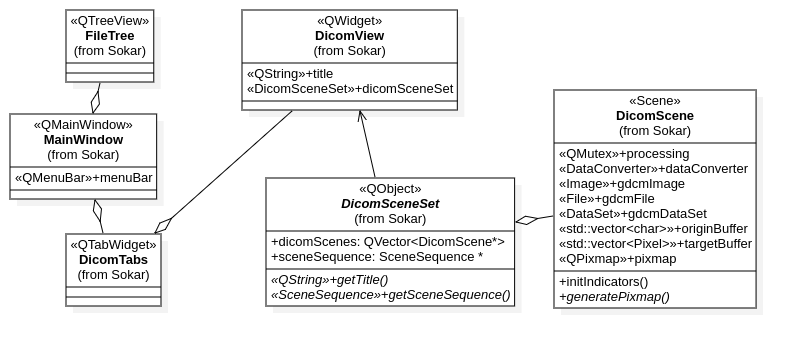
\includegraphics[width=\textwidth]{img/uml/global-sturcture.png}
    \caption{Diagram klas UML globalnej struktury programu.}
    \label{fig:uml-global-sturcture}
\end{figure}
